\documentclass[11pt,a4paper]{report}
\usepackage[textwidth=37em,vmargin=30mm]{geometry}
\usepackage{calc,xunicode,amsmath,amssymb,paralist,enumitem,tabu,booktabs,datetime2,xeCJK,xeCJKfntef,listings}
\usepackage{tocloft,fancyhdr,tcolorbox,xcolor,graphicx,eso-pic,xltxtra,xelatexemoji}

\newcommand{\envyear}[0]{2025}
\newcommand{\envdatestr}[0]{2025-08-19}
\newcommand{\envfinaldir}[0]{webdb/2025/20250819/final}

\usepackage[hidelinks]{hyperref}
\hypersetup{
    colorlinks=false,
    pdfpagemode=FullScreen,
    pdftitle={Web Digest - \envdatestr}
}

\setlength{\cftbeforechapskip}{10pt}
\renewcommand{\cftchapfont}{\rmfamily\bfseries\large\raggedright}
\setlength{\cftbeforesecskip}{2pt}
\renewcommand{\cftsecfont}{\sffamily\small\raggedright}

\setdefaultleftmargin{2em}{2em}{1em}{1em}{1em}{1em}

\usepackage{xeCJK,xeCJKfntef}
\xeCJKsetup{PunctStyle=plain,RubberPunctSkip=false,CJKglue=\strut\hskip 0pt plus 0.1em minus 0.05em,CJKecglue=\strut\hskip 0.22em plus 0.2em}
\XeTeXlinebreaklocale "zh"
\XeTeXlinebreakskip = 0pt


\setmainfont{Brygada 1918}
\setromanfont{Brygada 1918}
\setsansfont{IBM Plex Sans}
\setmonofont{JetBrains Mono NL}
\setCJKmainfont{Noto Serif CJK SC}
\setCJKromanfont{Noto Serif CJK SC}
\setCJKsansfont{Noto Sans CJK SC}
\setCJKmonofont{Noto Sans CJK SC}

\setlength{\parindent}{0pt}
\setlength{\parskip}{8pt}
\linespread{1.15}

\lstset{
	basicstyle=\ttfamily\footnotesize,
	numbersep=5pt,
	backgroundcolor=\color{black!5},
	showspaces=false,
	showstringspaces=false,
	showtabs=false,
	tabsize=2,
	captionpos=b,
	breaklines=true,
	breakatwhitespace=true,
	breakautoindent=true,
	linewidth=\textwidth
}






\newcommand{\coverpic}[2]{
    % argv: itemurl, authorname
    Cover photo by #2~~(\href{#1}{#1})
}
\newcommand{\makeheader}[0]{
    \begin{titlepage}
        % \newgeometry{hmargin=15mm,tmargin=21mm,bmargin=12mm}
        \begin{center}
            
            \rmfamily\scshape
            \fontspec{BaskervilleF}
            \fontspec{Old Standard}
            \fontsize{59pt}{70pt}\selectfont
            WEB\hfill DIGEST
            
            \vfill
            % \vskip 30pt
            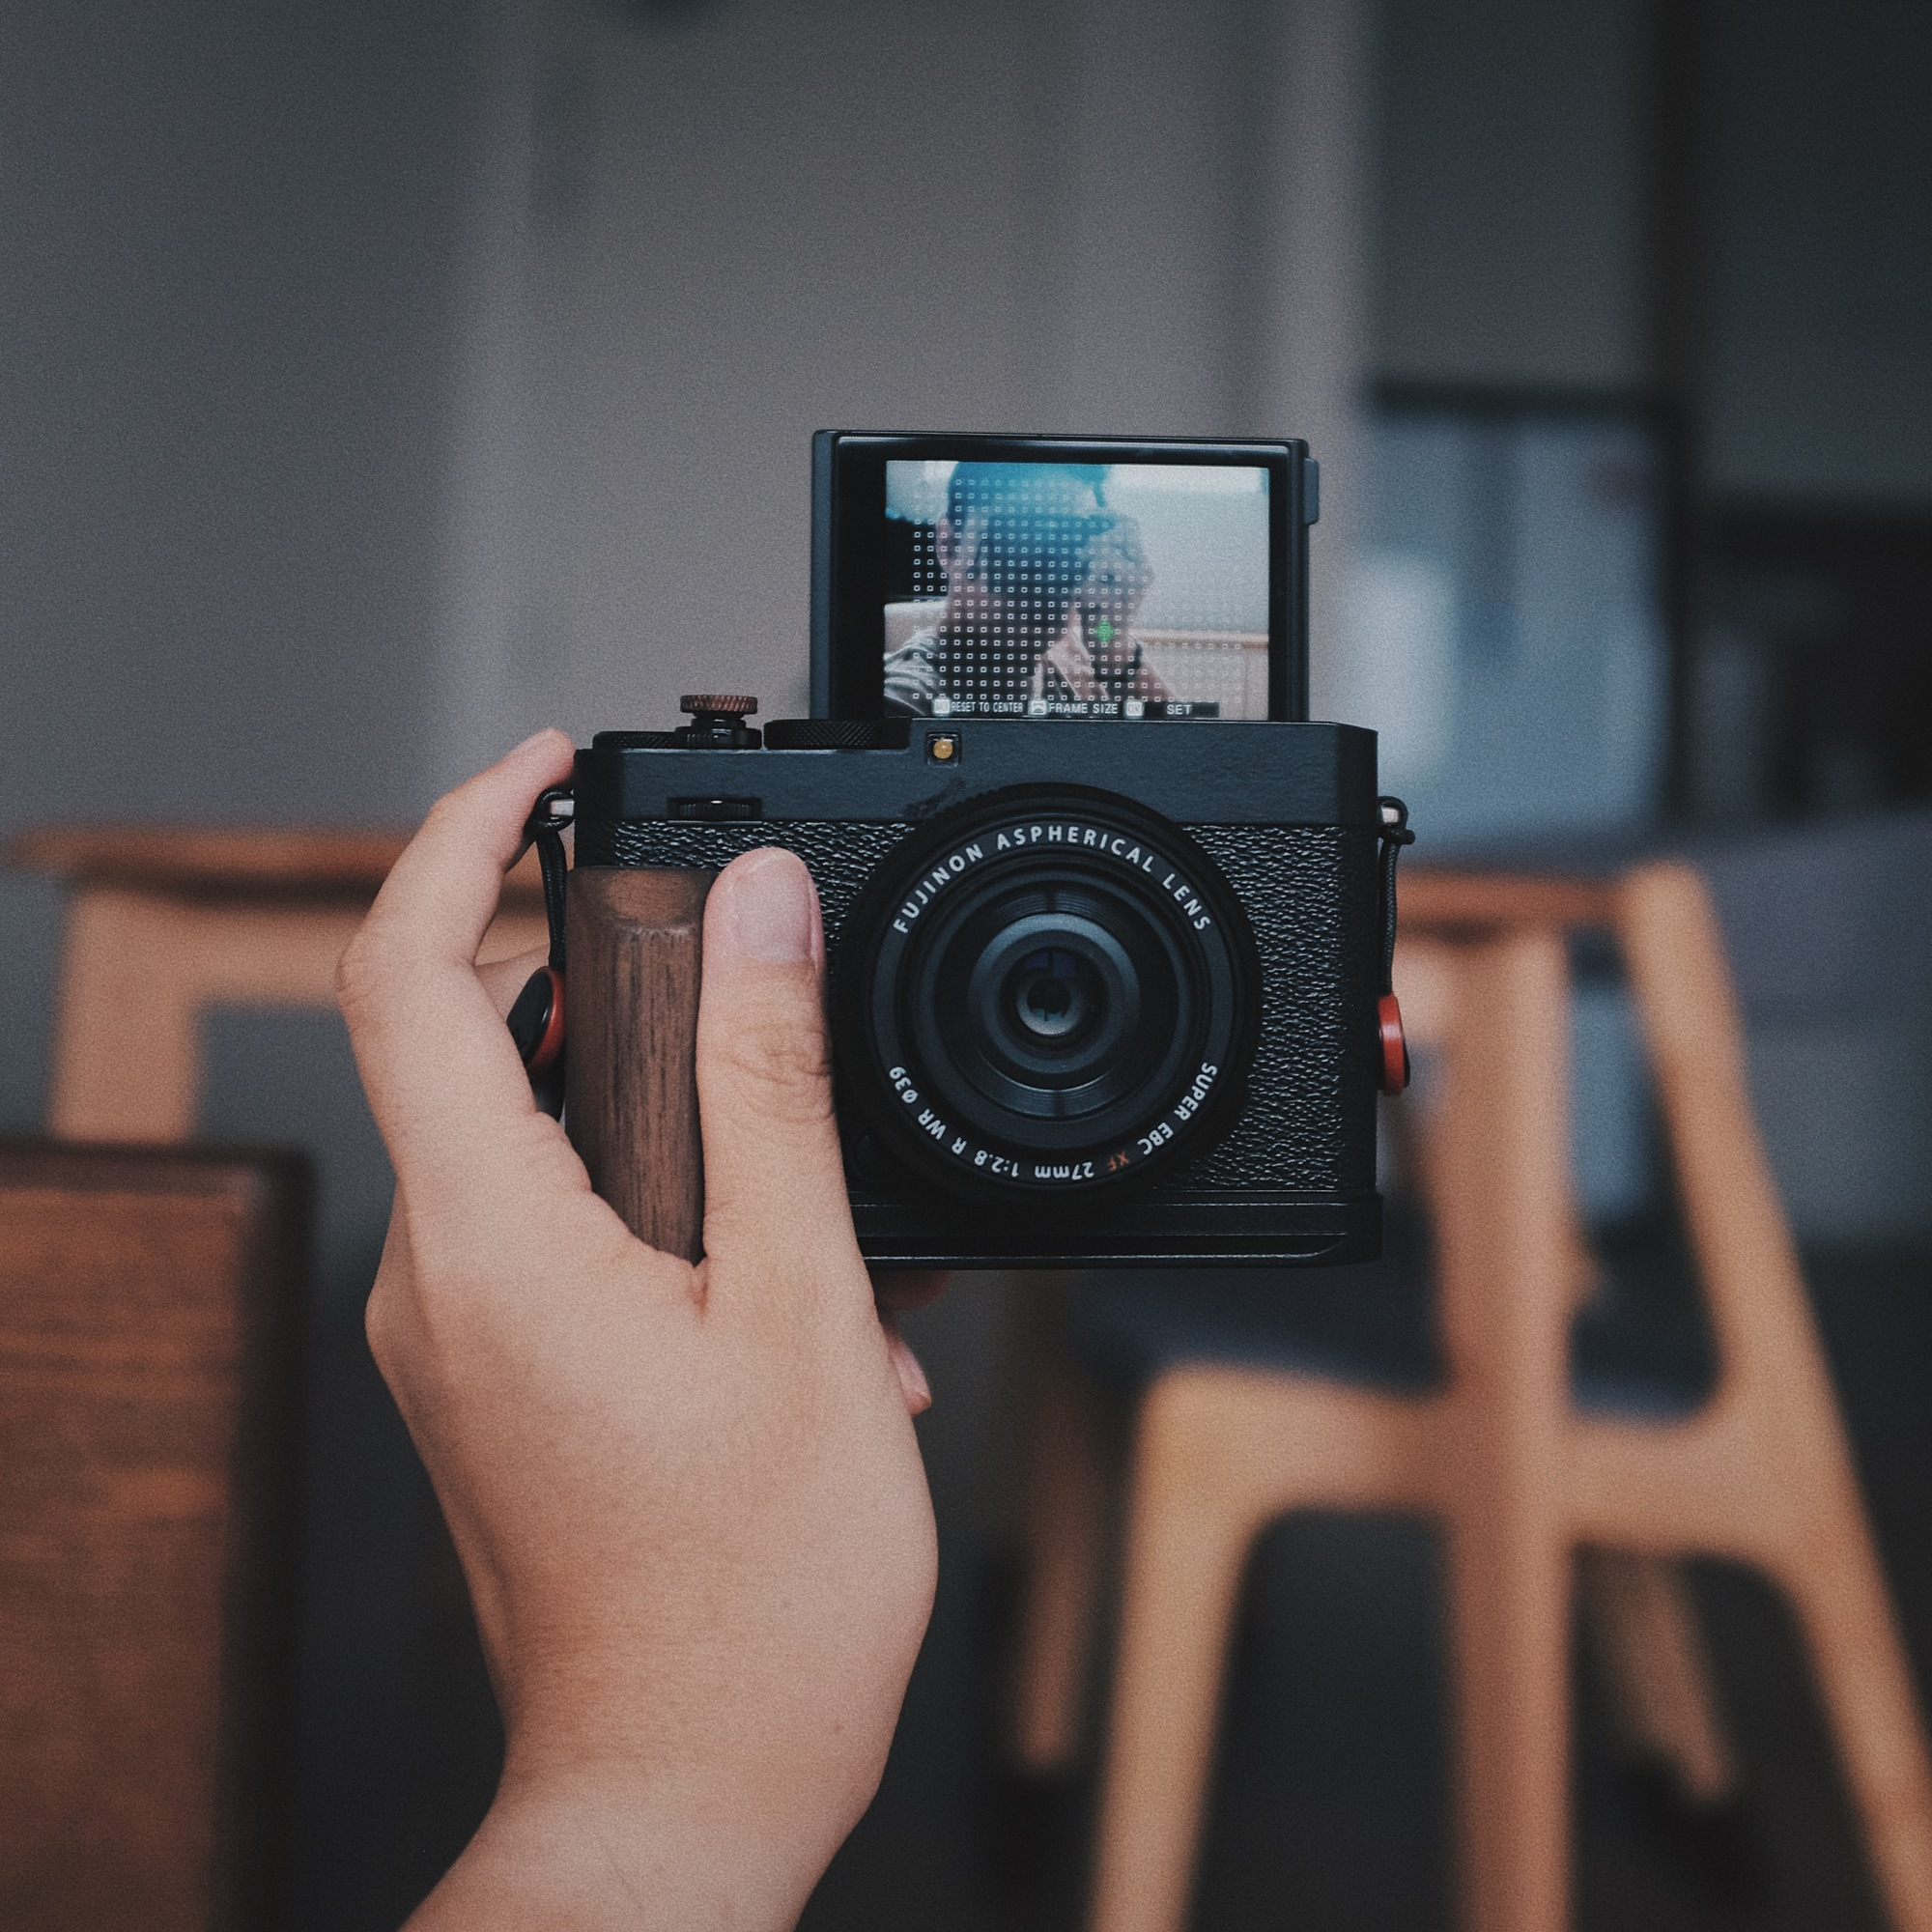
\includegraphics[width=\linewidth]{\envfinaldir/coverpic-prod.jpg}\par
            % \vskip 30pt
            \vfill

            \normalsize\rmfamily\scshape
            \copyright{} The Web Digest Project \hfill\large \envdatestr
        \end{center}
    \end{titlepage}
    % \restoregeometry
}
\newcommand{\simplehref}[1]{%
    \textcolor{blue!80!green}{\href{#1}{#1}}%
}
\renewcommand{\contentsname}{\center\Huge\sffamily\bfseries Contents\par\vskip 20pt}
\newcounter{ipartcounter}
\setcounter{ipartcounter}{0}
\newcommand{\ipart}[1]{
    % \vskip 20pt
    \clearpage
    \stepcounter{ipartcounter}
    \phantomsection
    \addcontentsline{toc}{chapter}{#1}
    % \begin{center}
    %     \Huge
    %     \sffamily\bfseries
    %     #1
    % \end{center}
    % \vskip 20pt plus 7pt
}
\newcounter{ichaptercounter}
\setcounter{ichaptercounter}{0}
\newcommand{\ichapter}[1]{
    % \vskip 20pt
    \clearpage
    \stepcounter{ichaptercounter}
    \phantomsection
    \addcontentsline{toc}{section}{\numberline{\arabic{ichaptercounter}}#1}
    \begin{center}
        \Huge
        \sffamily\bfseries
        #1
    \end{center}
    \vskip 20pt plus 7pt
}
\newcommand{\entrytitlefont}[1]{\subsection*{\raggedright\Large\sffamily\bfseries#1}}
\newcommand{\entryitemGeneric}[2]{
    % argv: title, url
    \parbox{\linewidth}{
        \entrytitlefont{#1}\par\vskip 5pt
        \footnotesize\ttfamily\mdseries
        \simplehref{#2}
    }\vskip 11pt plus 11pt minus 1pt
}
\newcommand{\entryitemGithub}[3]{
    % argv: title, url, desc
    \parbox{\linewidth}{
        \entrytitlefont{#1}\par\vskip 5pt
        \footnotesize\ttfamily\mdseries
        \simplehref{#2}\par\vskip 5pt
        \small\rmfamily\mdseries#3
    }\vskip 11pt plus 11pt minus 1pt
}
\newcommand{\entryitemAp}[3]{
    % argv: title, url, desc
    \parbox{\linewidth}{
        \entrytitlefont{#1}\par\vskip 5pt
        \footnotesize\ttfamily\mdseries
        \simplehref{#2}\par\vskip 5pt
        \small\rmfamily\mdseries#3
    }\vskip 11pt plus 11pt minus 1pt
}
\newcommand{\entryitemHackernews}[3]{
    % argv: title, hnurl, rawurl
    % \parbox{\linewidth}{
    %     \entrytitlefont{#1}\par\vskip 5pt
    %     \footnotesize\ttfamily\mdseries
    %     \simplehref{#3}\par
    %     \textcolor{black!50}{\href{#2}{#2}}
    % }\vskip 11pt plus 11pt minus 1pt
    \begin{minipage}{\linewidth}
            \entrytitlefont{#1}\par\vskip 5pt
            \footnotesize\ttfamily\mdseries
            \simplehref{#3}\par
            \textcolor{black!50}{\href{#2}{#2}}
    \end{minipage}\par\vskip 11pt plus 11pt minus 1pt
}







\begin{document}

\makeheader

\tableofcontents\clearpage




\ipart{Developers}
\ichapter{Hacker News}
\entryitemTwoLinks{Newsmax agrees to pay \$67M in defamation case over bogus 2020 election claims}{https://news.ycombinator.com/item?id=44945925}{https://apnews.com/article/dominion-voting-newsmax-defamation-trump-2020-3b2366dfdae3a8432afe822bf14fe1ef}

\entryitemTwoLinks{Obsidian Bases}{https://news.ycombinator.com/item?id=44945532}{https://help.obsidian.md/bases}

\entryitemTwoLinks{GenAI FOMO has spurred businesses to light nearly \$40B on fire}{https://news.ycombinator.com/item?id=44944620}{https://www.theregister.com/2025/08/18/generative\_ai\_zero\_return\_95\_percent/}

\entryitemTwoLinks{T-Mobile claimed selling location data without consent is legal–judges disagree}{https://news.ycombinator.com/item?id=44944291}{https://arstechnica.com/tech-policy/2025/08/t-mobile-claimed-selling-location-data-without-consent-is-legal-judges-disagree/}

\entryitemTwoLinks{Left to Right Programming}{https://news.ycombinator.com/item?id=44942936}{https://graic.net/p/left-to-right-programming}

\entryitemTwoLinks{Show HN: Whispering – Open-source, local-first dictation you can trust}{https://news.ycombinator.com/item?id=44942731}{https://github.com/epicenter-so/epicenter/tree/main/apps/whispering}

\entryitemTwoLinks{My Retro TVs}{https://news.ycombinator.com/item?id=44942602}{https://www.myretrotvs.com/}

\entryitemTwoLinks{Anna's Archive: An Update from the Team}{https://news.ycombinator.com/item?id=44942501}{https://annas-archive.org/blog/an-update-from-the-team.html}

\entryitemTwoLinks{Who Invented Backpropagation?}{https://news.ycombinator.com/item?id=44941963}{https://people.idsia.ch/~juergen/who-invented-backpropagation.html}

\entryitemTwoLinks{The road that killed Legend Jenkins was working as designed}{https://news.ycombinator.com/item?id=44941766}{https://www.strongtowns.org/journal/2025/8/18/the-road-that-killed-legend-jenkins-was-working-exactly-as-designed}

\entryitemTwoLinks{Counter-Strike: A billion-dollar game built in a dorm room}{https://news.ycombinator.com/item?id=44941369}{https://www.nytimes.com/2025/08/18/arts/counter-strike-half-life-minh-le.html}

\entryitemTwoLinks{95\% of AI Pilots Failing}{https://news.ycombinator.com/item?id=44941118}{https://fortune.com/2025/08/18/mit-report-95-percent-generative-ai-pilots-at-companies-failing-cfo/}

\entryitemTwoLinks{AI is predominantly replacing outsourced, offshore workers}{https://news.ycombinator.com/item?id=44940944}{https://www.axios.com/2025/08/18/ai-jobs-layoffs}

\entryitemTwoLinks{Class-action suit claims Otter AI records private work conversations}{https://news.ycombinator.com/item?id=44940554}{https://www.npr.org/2025/08/15/g-s1-83087/otter-ai-transcription-class-action-lawsuit}

\entryitemTwoLinks{FFmpeg Assembly Language Lessons}{https://news.ycombinator.com/item?id=44940485}{https://github.com/FFmpeg/asm-lessons}

\entryitemTwoLinks{Texas law gives grid operator power to disconnect data centers during crisis}{https://news.ycombinator.com/item?id=44940416}{https://www.utilitydive.com/news/texas-law-gives-grid-operator-power-to-disconnect-data-centers-during-crisi/751587/}

\entryitemTwoLinks{Vibe coding tips and tricks}{https://news.ycombinator.com/item?id=44940089}{https://github.com/awslabs/mcp/blob/main/VIBE\_CODING\_TIPS\_TRICKS.md}

\entryitemTwoLinks{When you're asking AI chatbots for answers, they're data-mining you}{https://news.ycombinator.com/item?id=44939660}{https://www.theregister.com/2025/08/18/opinion\_column\_ai\_surveillance/}

\entryitemTwoLinks{LLMs and coding agents are a security nightmare}{https://news.ycombinator.com/item?id=44939331}{https://garymarcus.substack.com/p/llms-coding-agents-security-nightmare}

\entryitemTwoLinks{Website is served from nine Neovim buffers on my old ThinkPad}{https://news.ycombinator.com/item?id=44939324}{https://vim.gabornyeki.com/}\ichapter{Phoronix}
\entryitemGeneric{\hskip 0pt{}AMD "GFX1250" To Double The Number Of User SGPRs}{https://www.phoronix.com/news/AMD-GFX1250-32-User-SGPRs}

\entryitemGeneric{\hskip 0pt{}AMD ZenDNN 5.1 Released For Enhancing AI Inference Performance On EPYC CPUs}{https://www.phoronix.com/news/AMD-ZenDNN-5.1}

\entryitemGeneric{\hskip 0pt{}Kdenlive 25.08 Preps For Future Hardware Acceleration Features}{https://www.phoronix.com/news/Kdenlive-25.08-Released}

\entryitemGeneric{\hskip 0pt{}Git 2.51 Released With More Changes Preparing For Git 3.0}{https://www.phoronix.com/news/Git-2.51-Released}

\entryitemGeneric{\hskip 0pt{}A Deep Dive Into The Power \& Thermals For The Framework Desktop With AMD Ryzen AI Max}{https://www.phoronix.com/review/framework-desktop-power}

\entryitemGeneric{\hskip 0pt{}AMD Posts Latest Linux Patches For Improving S5 Power Consumption}{https://www.phoronix.com/news/AMD-S5-Power-Optimizations-v6}

\entryitemGeneric{\hskip 0pt{}Firefox 142 Now Available - Allows Browser Extensions/Add-Ons To Use AI LLMs}{https://www.phoronix.com/news/Firefox-142-Extensions-AI-LLMs}

\entryitemGeneric{\hskip 0pt{}GNOME 49 Merges Late Mutter Change To Help Cursor Responsiveness With VRR}{https://www.phoronix.com/news/GNOME-49-VRR-Cursor}

\entryitemGeneric{\hskip 0pt{}Illumos Cafe Hopes To Reinvigorate Interest In Illumos/OpenSolaris Derived Platforms}{https://www.phoronix.com/news/Illumos-Cafe}


\ipart{Developers~~~~(zh-Hans)}
\ichapter{Solidot}
\entryitemGeneric{\hskip 0pt{}一种蛋白质在人体中传递衰老信号}{https://www.solidot.org/story?sid=82070}

\entryitemGeneric{\hskip 0pt{}2025 年雨果奖宣布}{https://www.solidot.org/story?sid=82069}

\entryitemGeneric{\hskip 0pt{}FFmpeg 迁移到 Forgejo}{https://www.solidot.org/story?sid=82068}

\entryitemGeneric{\hskip 0pt{}克罗地亚将数字游民签证有效期延长至三年}{https://www.solidot.org/story?sid=82067}

\entryitemGeneric{\hskip 0pt{}今年前七个月电动汽车销量同比增长 27\%}{https://www.solidot.org/story?sid=82066}

\entryitemGeneric{\hskip 0pt{}PuTTY 有了新官网}{https://www.solidot.org/story?sid=82065}

\entryitemGeneric{\hskip 0pt{}德国最高法院部分推翻广告屏蔽工具不侵犯版权判决}{https://www.solidot.org/story?sid=82064}\ichapter{V2EX}
\entryitemGeneric{\hskip 0pt{}[分享创造] [工具自荐] 花了几天用 claude code 做了个解梦网站。免费用!}{https://www.v2ex.com/t/1153333}

\entryitemGeneric{\hskip 0pt{}[汽车] 你们是怎么确定保养要做的项目的}{https://www.v2ex.com/t/1153332}

\entryitemGeneric{\hskip 0pt{}[程序员] 找人开发一个检测是否为 Ai 图的模型要多少费用}{https://www.v2ex.com/t/1153331}

\entryitemGeneric{\hskip 0pt{}[生活] 看完 1781,分享下我的 3409 天}{https://www.v2ex.com/t/1153330}

\entryitemGeneric{\hskip 0pt{}[问与答] 怎么理解``你戾气真重''}{https://www.v2ex.com/t/1153329}

\entryitemGeneric{\hskip 0pt{}[程序员] 你们在备份数据时会暂停服务以保持数据的一致性吗?}{https://www.v2ex.com/t/1153328}

\entryitemGeneric{\hskip 0pt{}[macOS] Beta7 尝鲜}{https://www.v2ex.com/t/1153327}

\entryitemGeneric{\hskip 0pt{}[Apple] 如何禁止 Siri 打电话?}{https://www.v2ex.com/t/1153326}

\entryitemGeneric{\hskip 0pt{}[汽车] 交强险如果过期没买有什么后果}{https://www.v2ex.com/t/1153325}

\entryitemGeneric{\hskip 0pt{}[问与答] 有家畜生一样的邻居怎么办?}{https://www.v2ex.com/t/1153324}

\entryitemGeneric{\hskip 0pt{}[分享创造] Chrome 插件:推特 Profile 扩展菜单和隐藏窗口功能}{https://www.v2ex.com/t/1153323}

\entryitemGeneric{\hskip 0pt{}[职场话题] 个人目前很迷茫,求老哥指点下方向}{https://www.v2ex.com/t/1153322}

\entryitemGeneric{\hskip 0pt{}[SQLite] 分享适合高并发场景的 SQLite 设置}{https://www.v2ex.com/t/1153321}

\entryitemGeneric{\hskip 0pt{}[OpenAI] 现在本地部署了一个 gpt-oss,有什么好的提示词可以解除它的道德限制吗,可以搞成人相关的东西的}{https://www.v2ex.com/t/1153319}

\entryitemGeneric{\hskip 0pt{}[站长] 收网站:下载站、游戏站、编程站、资源站、教程资源等等}{https://www.v2ex.com/t/1153318}

\entryitemGeneric{\hskip 0pt{}[Solana] 1781 天后\$V2EX 能到什么价位?能到\$17.82 嘛?}{https://www.v2ex.com/t/1153317}

\entryitemGeneric{\hskip 0pt{}[Cloudflare] 网站上 cloudflare 之后的奇怪流量都是哪里来的}{https://www.v2ex.com/t/1153316}

\entryitemGeneric{\hskip 0pt{}[数学] 猜不重复 4 位数,只能回答同位命中多少个,有无最快必胜办法?}{https://www.v2ex.com/t/1153315}

\entryitemGeneric{\hskip 0pt{}[职场话题] 怎么克服找工作面试的恐惧?}{https://www.v2ex.com/t/1153314}

\entryitemGeneric{\hskip 0pt{}[职场话题] 合同续签,五险一金缴纳基数,亏大了}{https://www.v2ex.com/t/1153313}

\entryitemGeneric{\hskip 0pt{}[分享创造] 写了个基于 NPM 的插件系统}{https://www.v2ex.com/t/1153312}

\entryitemGeneric{\hskip 0pt{}[游戏] 云风推荐的桌游 Deep Future 到底是什么游戏?怎么玩?}{https://www.v2ex.com/t/1153311}

\entryitemGeneric{\hskip 0pt{}[ACG] 有人知道遮天的解说大帝为什么没了,还会回来么}{https://www.v2ex.com/t/1153310}

\entryitemGeneric{\hskip 0pt{}[天黑以后] 20250818 午夜俱乐部}{https://www.v2ex.com/t/1153309}

\entryitemGeneric{\hskip 0pt{}[生活] 都来说说国内银行卡被限额的那些事}{https://www.v2ex.com/t/1153307}

\entryitemGeneric{\hskip 0pt{}[职场话题] 后悔的一次跳槽决定}{https://www.v2ex.com/t/1153306}

\entryitemGeneric{\hskip 0pt{}[分享创造] 脚本分享, SpeedUp 长按空格倍速播放视频}{https://www.v2ex.com/t/1153304}

\entryitemGeneric{\hskip 0pt{}[电影] 《碟中谍 8》中的代码片段}{https://www.v2ex.com/t/1153303}

\entryitemGeneric{\hskip 0pt{}[问与答] win 用户切换到 mac 的几个问题想请教一下}{https://www.v2ex.com/t/1153302}

\entryitemGeneric{\hskip 0pt{}[VPS] 请兄弟们推荐 VPS}{https://www.v2ex.com/t/1153301}

\entryitemGeneric{\hskip 0pt{}[YouTube] 油管这么牛比么?这是自动翻译音轨,还是人工的?}{https://www.v2ex.com/t/1153300}

\entryitemGeneric{\hskip 0pt{}[问与答] App 对接聚合广告}{https://www.v2ex.com/t/1153298}

\entryitemGeneric{\hskip 0pt{}[前端开发] 请教大佬 FluentUI Toast 不显示的问题}{https://www.v2ex.com/t/1153297}

\entryitemGeneric{\hskip 0pt{}[问与答] 各位 Gopher 的 IDE 是什么? VSCode V.S. GoLand}{https://www.v2ex.com/t/1153294}

\entryitemGeneric{\hskip 0pt{}[iOS] 今天晚上或者明天有 iOSBeta7 吗?}{https://www.v2ex.com/t/1153292}

\entryitemGeneric{\hskip 0pt{}[分享创造] 用 Claude Code 做了一个图片增强和去背景网站(免费用)}{https://www.v2ex.com/t/1153291}

\entryitemGeneric{\hskip 0pt{}[Linux] ubuntu/debian 如何才能把 lvm thin 逻辑卷上的分区作为根文件系统?}{https://www.v2ex.com/t/1153290}

\entryitemGeneric{\hskip 0pt{}[问与答] MUJI 的硅胶锅铲有人用过吗,种草了}{https://www.v2ex.com/t/1153289}

\entryitemGeneric{\hskip 0pt{}[数据库] 不限语言,你觉得最好用的框架和 ORM 是什么?}{https://www.v2ex.com/t/1153288}

\entryitemGeneric{\hskip 0pt{}[macOS] 请教 mac 能部署生成图片和视频的本地 ai 么?}{https://www.v2ex.com/t/1153287}

\entryitemGeneric{\hskip 0pt{}[生活] 看完 1781 的校园爱情分手贴,想到十年前自己的小故事}{https://www.v2ex.com/t/1153285}

\entryitemGeneric{\hskip 0pt{}[程序员] [超越 Manus] 超级智能体《imini》聚合 23 款全球 AI 大模型 kimi、GPT、Gemin、Grok、Claude...}{https://www.v2ex.com/t/1153283}

\entryitemGeneric{\hskip 0pt{}[Windows] win11 更新会导致 SSD 掉盘?}{https://www.v2ex.com/t/1153281}

\entryitemGeneric{\hskip 0pt{}[奇思妙想] 在学钢琴或者家里有人弹钢琴的看过来-是不是需要这样一个钢琴助手?}{https://www.v2ex.com/t/1153277}

\entryitemGeneric{\hskip 0pt{}[问与答] 求大佬帮忙推荐装机配置(锁定 983/783+5070ti)!}{https://www.v2ex.com/t/1153276}

\entryitemGeneric{\hskip 0pt{}[问与答] 蹭蹭 1781 天热度,你每个月会给女朋友花多少钱?}{https://www.v2ex.com/t/1153275}

\entryitemGeneric{\hskip 0pt{}[云计算] BUYPASS 终止了 SSL 证书的签发}{https://www.v2ex.com/t/1153273}

\entryitemGeneric{\hskip 0pt{}[问与答] 都是搞技术的、没有玩权力的?}{https://www.v2ex.com/t/1153272}

\entryitemGeneric{\hskip 0pt{}[生活] 这个孙宇晨就像小说的主角,简直开挂了一样}{https://www.v2ex.com/t/1153271}

\entryitemGeneric{\hskip 0pt{}[生活] 2351 天,时间会抹平一切}{https://www.v2ex.com/t/1153270}


\ipart{Generic News}







\clearpage
\leavevmode\vfill
\footnotesize

Copyright \copyright{} 2023-2025 Neruthes and other contributors.

This document is published with CC BY-NC-ND 4.0 license.

The entries listed in this newsletter may be copyrighted by their respective creators.

This newsletter is generated by the Web Digest project.

The newsletters are also delivered via Telegram channel \CJKunderline{\href{https://t.me/webdigestchannel}{https://t.me/webdigestchannel}}.\\
RSS feed is available at \CJKunderline{\href{https://webdigest.pages.dev/rss.xml}{https://webdigest.pages.dev/rss.xml}}.

This newsletter is available in PDF at
\CJKunderline{\href{https://webdigest.pages.dev/}{https://webdigest.pages.dev/}}.

The source code being used to generate this newsletter is available at\\
\CJKunderline{\href{https://github.com/neruthes/webdigest}{https://github.com/neruthes/webdigest}}.

This newsletter is also available in
\CJKunderline{\href{http://webdigest.pages.dev/readhtml/\envyear/WebDigest-20250819.html}{HTML}} and
\CJKunderline{\href{https://github.com/neruthes/webdigest/blob/master/markdown/\envyear/WebDigest-20250819.md}{Markdown}}.


\coverpic{https://unsplash.com/photos/photo-of-a-women-holding-three-balloon-close-up-photography-\_U3u\_8zsiIs}{roland deason}


\end{document}
